\documentclass{article}
\usepackage[utf8]{inputenc}

\title{\textbf{CSE 4701}\\ Project 1, Part 2}
\author{Mike Medved}
\date{October 4th, 2023}

\usepackage{graphicx}
\usepackage{amsthm}
\usepackage{amssymb} 
\usepackage{amsmath}
\usepackage{caption}
\usepackage{listings}
\usepackage{multirow, tabularx}
\usepackage[margin=1in]{geometry} 
\usepackage[table,xcdraw]{xcolor}
\usepackage{enumitem}
\newlist{parlist}{enumerate}{1}
\setlist[parlist]{label=(\alph*),wide=0pt,topsep=0pt}

% changes title name for the table of contents
\renewcommand*\contentsname{Table of Contents}

% makes sections unnumbered and hides numbers from table of contents
\setcounter{secnumdepth}{0}

\newcolumntype{C}{>{\centering\arraybackslash}X}
\NewExpandableDocumentCommand\mcc{O{1}m}{\multicolumn{#1}{c}{#2}}

\definecolor{codegreen}{rgb}{0,0.6,0}
\definecolor{codegray}{rgb}{0.5,0.5,0.5}
\definecolor{codepurple}{HTML}{C42043}
\definecolor{backcolour}{HTML}{F2F2F2}
\definecolor{bookColor}{cmyk}{0,0,0,0.90}  
\color{bookColor}

\lstset{upquote=true}

\lstdefinestyle{mystyle}{
    backgroundcolor=\color{backcolour},   
    commentstyle=\color{codegreen},
    keywordstyle=\color{codepurple},
    numberstyle=\numberstyle,
    stringstyle=\color{codepurple},
    basicstyle=\scriptsize\ttfamily,
    breakatwhitespace=false,
    breaklines=true,
    postbreak=\mbox{\textcolor{red}{$\hookrightarrow$}\space},
    captionpos=b,
    keepspaces=true,
    numbers=left,
    numbersep=10pt,
    showspaces=false,
    showstringspaces=false,
    showtabs=false,
}
\lstset{style=mystyle}

\newcommand\numberstyle[1]{%
    \footnotesize
    \color{codegray}%
    \ttfamily
    \ifnum#1<10 0\fi#1 |%
}

\def\ojoin{\setbox0=\hbox{$\bowtie$}%
  \rule[-.02ex]{.25em}{.4pt}\llap{\rule[\ht0]{.25em}{.4pt}}}
\def\leftouterjoin{\mathbin{\ojoin\mkern-5.8mu\bowtie}}
\def\rightouterjoin{\mathbin{\bowtie\mkern-5.8mu\ojoin}}
\def\fullouterjoin{\mathbin{\ojoin\mkern-5.8mu\bowtie\mkern-5.8mu\ojoin}}

\begin{document}

\maketitle

\tableofcontents

\newpage
\section{Part 1, Modifying the Publisher Table}

\subsection{Last Assignment State}

Here is the state as it was left from the previous assignment:

\begin{figure}[!h]
    \centering
    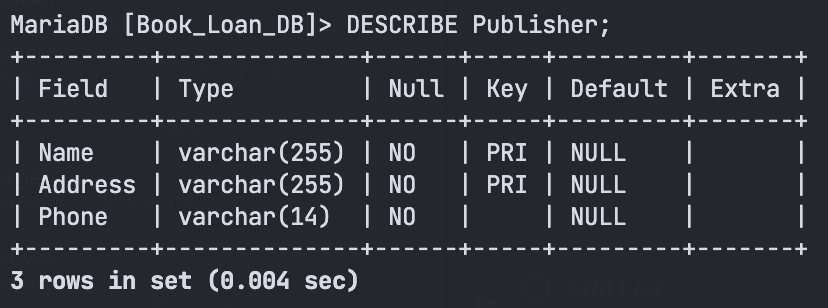
\includegraphics[scale=0.65]{images/q1-a-describe-publisher.png}
    \caption{Last Assignment State}
    \label{fig:last_state}
\end{figure}

\subsection{Adding the New Column}

We can use the \textit{ALTER} command to add another column to the \textit{Publisher} table. The command is as follows:

\begin{lstlisting}[ language=SQL,
    deletekeywords={IDENTITY},
    deletekeywords={[2]INT},
    morekeywords={clustered},
    framesep=8pt,
    xleftmargin=40pt,
    framexleftmargin=40pt,
    frame=tb,
    framerule=0pt ]
ALTER TABLE Publisher ADD COLUMN City VARCHAR(255) NOT NULL;
\end{lstlisting}

$\hfill \break$
As a result, we get the following table schema after executing the above command:

\begin{figure}[!h]
    \centering
    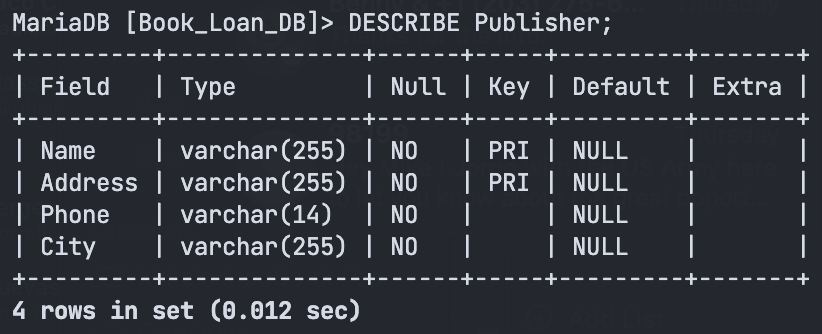
\includegraphics[scale=0.65]{images/q1-bc-add-col-publisher.png}
    \caption{Table Schema After Adding New Column}
    \label{fig:q1_after_adding}
\end{figure}

$\hfill \break$
Additionally, this is the result we get when we execute a \textit{SELECT} all operation against the table:

\begin{figure}[!h]
    \centering
    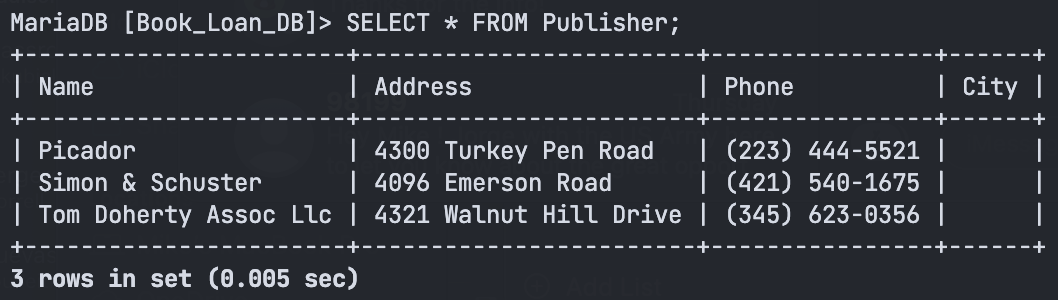
\includegraphics[scale=0.65]{images/q1-c-select-publisher.png}
    \caption{Select Operation Result}
    \label{fig:q1_select_all}
\end{figure}

$\hfill \break$
Here, we can see that the new column is added to the table, and all of the values are blank, not \textit{NULL}.

\section{Part 2, Emptying the Tables}

\subsection{Deleting the Records}

We can delete all records from the tables in our database by using the \textit{DELETE FROM \text{[table]}} syntax as seen below:

\begin{lstlisting}[ language=SQL,
    deletekeywords={IDENTITY},
    deletekeywords={[2]INT},
    morekeywords={clustered},
    framesep=8pt,
    xleftmargin=40pt,
    framexleftmargin=40pt,
    frame=tb,
    framerule=0pt ]
DELETE FROM Book_Authors;
DELETE FROM Book_Copies;
DELETE FROM Book_Loans;
DELETE FROM Book;
DELETE FROM Borrower;
DELETE FROM Library_Branch;
DELETE FROM Publisher;
\end{lstlisting}

$\hfill \break$
Do note, we need to delete records from tables in a specific order as to not violate foreign key constraints.

\begin{figure}[!h]
    \centering
    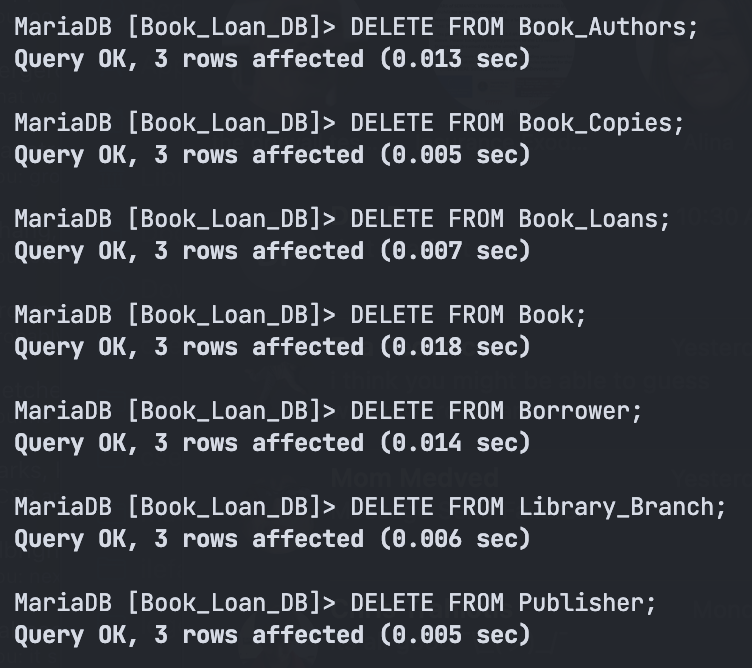
\includegraphics[scale=0.5]{images/q2-delete-records.png}
    \caption{Table Schema After Adding New Column}
    \label{fig:q2_delete_records}
\end{figure}

\subsection{Verifying Deletion}

Once all of the \textit{DELETE} commands are executed, we can use \textit{SELECT} to verify all data has been removed.

\begin{figure}[!h]
    \centering
    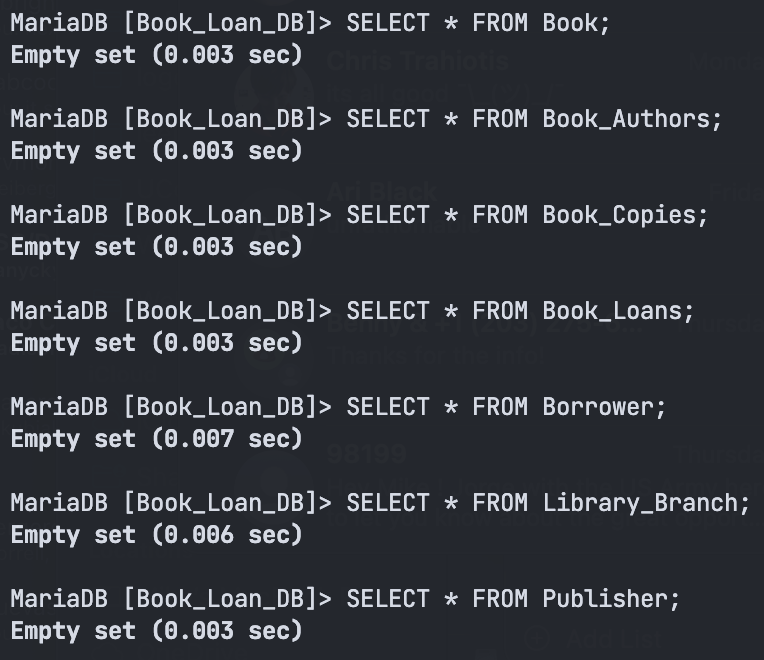
\includegraphics[scale=0.5]{images/q2-select-tables.png}
    \caption{Select Operation Result}
    \label{fig:q2_select_tables}
\end{figure}

\section{Part 3, Importing CSV-Formatted Data}

\subsection{Importing the Data}

We can use this command template to import all of the obtained CSV files into their respective tables.

\begin{lstlisting}[language=SQL,
    deletekeywords={IDENTITY},
    deletekeywords={[2]INT},
    morekeywords={clustered,load,data,infile,fields,terminated,enclosed,lines},
    framesep=8pt,
    xleftmargin=40pt,
    framexleftmargin=40pt,
    frame=tb,
    framerule=0pt ]
LOAD DATA LOCAL INFILE 
    ['/path/to/csv']
INTO TABLE
    [table] 
FIELDS TERMINATED BY ',' ENCLOSED BY '"'
LINES TERMINATED BY '\r\n';
\end{lstlisting}

\subsection{Resultant Tuple Counts}

After importing all of the data from the provided CSV files, we can use the \textit{SELECT} command to count the amount of rows in each table. The command template, and totals are shown below:

\begin{lstlisting}[language=SQL,
    deletekeywords={IDENTITY},
    deletekeywords={[2]INT},
    morekeywords={clustered},
    framesep=8pt,
    xleftmargin=40pt,
    framexleftmargin=40pt,
    frame=tb,
    framerule=0pt ]
SELECT COUNT(*) FROM [table];
\end{lstlisting}

\begin{figure}[!h]
    \centering
    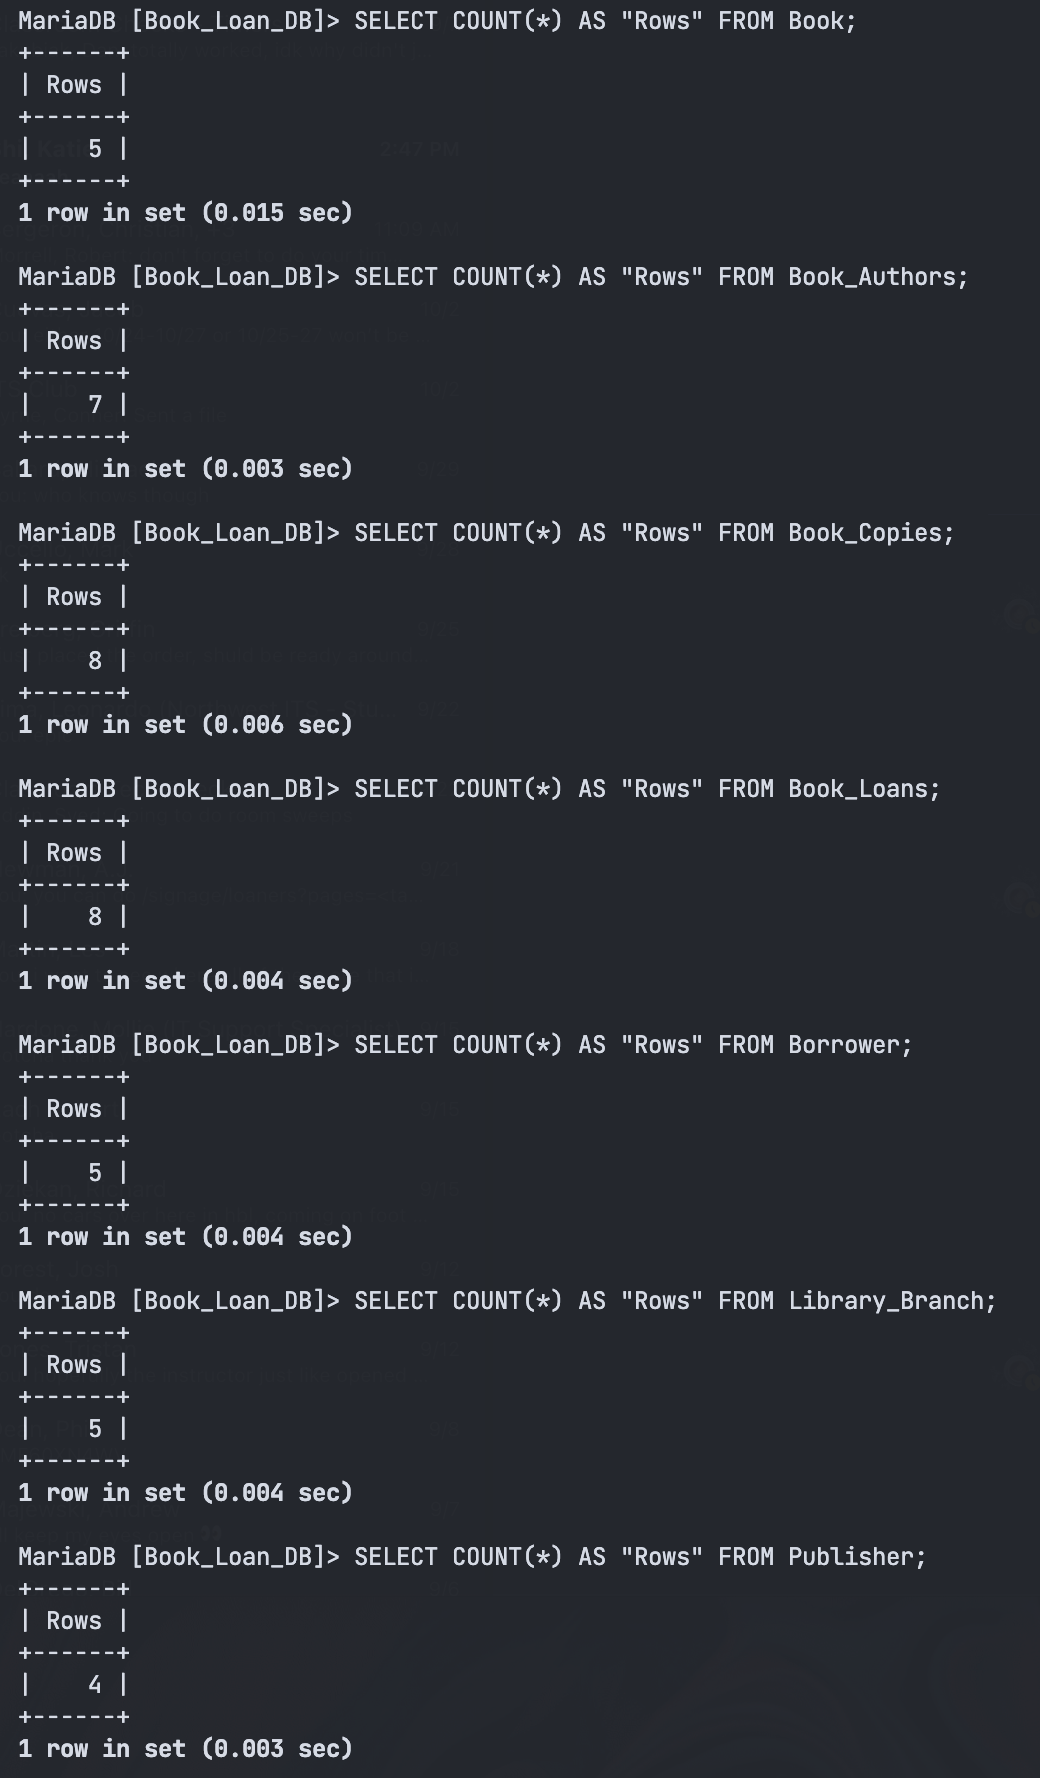
\includegraphics[scale=0.425]{images/q3-import-results.png}
    \caption{Tuple Counts}
    \label{fig:q3_tuple_counts}
\end{figure}

\section{Part 4, Complex Query Exercises}

\subsection{a) Copies of a book at one branch}

\textit{How many copies of the book `The Lost Tribe' are owned by branch `Sharpstown'?}

\begin{lstlisting}[language=SQL,
    deletekeywords={IDENTITY},
    deletekeywords={[2]INT},
    morekeywords={clustered},
    framesep=8pt,
    xleftmargin=40pt,
    framexleftmargin=40pt,
    frame=tb,
    framerule=0pt ]
SELECT No_of_copies FROM Book_Copies WHERE Book_id="B1" AND Branch_id="BR1";
\end{lstlisting}

\begin{figure}[!h]
    \centering
    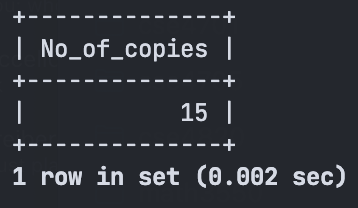
\includegraphics[scale=0.6]{images/q4-a-results.png}
    \caption{Number of Copies of `The Lost Tribe' at `Sharpstown'}
    \label{fig:q4_a_copies_of_book}
\end{figure}

\subsection{b) Copies of a book at all branches}

\textit{How many copies of the book `The Lost Tribe' are owned by each branch?}

\begin{lstlisting}[language=SQL,
    deletekeywords={IDENTITY},
    deletekeywords={[2]INT},
    morekeywords={clustered},
    framesep=8pt,
    xleftmargin=40pt,
    framexleftmargin=40pt,
    frame=tb,
    framerule=0pt ]
SELECT Branch_id, No_of_copies FROM Book_Copies WHERE Book_id = "B1"; 
\end{lstlisting}

\begin{figure}[!h]
    \centering
    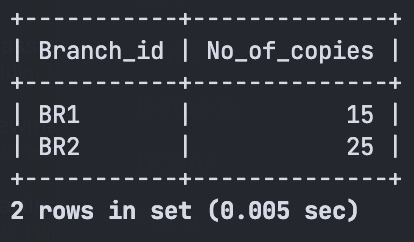
\includegraphics[scale=0.6]{images/q4-b-results.png}
    \caption{Number of Copies of `The Lost Tribe' at All Branches}
    \label{fig:q4_b_copies_of_book}
\end{figure}

\subsection{c) Borrowers with no books checked out}

\textit{Retrieve the names of all borrowers who do not have any books checked out.}

\begin{lstlisting}[language=SQL,
    deletekeywords={IDENTITY},
    deletekeywords={[2]INT},
    morekeywords={clustered},
    framesep=8pt,
    xleftmargin=40pt,
    framexleftmargin=40pt,
    frame=tb,
    framerule=0pt ]
SELECT 
    b.Card_no,
    b.Name
FROM Borrower b
LEFT JOIN Book_Loans l
    ON b.Card_no = l.Card_no
WHERE l.Card_no IS NULL; 
\end{lstlisting}

\begin{figure}[!h]
    \centering
    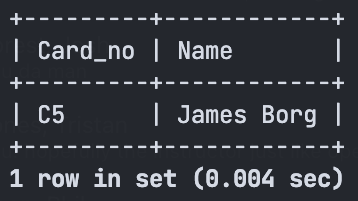
\includegraphics[scale=0.6]{images/q4-c-results.png}
    \caption{Borrowers with No Books Checked Out}
    \label{fig:q4_c_borrowers}
\end{figure}

\newpage
\subsection{d) Information about all books loaned on 1/3/2023}

\textit{Assume today is 1/3/2023. For each book that is loaned out from the Sharpstown branch,
retrieve the book title, the borrower's name, and the borrower's address.}

\begin{lstlisting}[language=SQL,
    deletekeywords={IDENTITY},
    deletekeywords={[2]INT},
    morekeywords={clustered},
    framesep=8pt,
    xleftmargin=40pt,
    framexleftmargin=40pt,
    frame=tb,
    framerule=0pt ]
SELECT
    b.Title,
    u.Name,
    u.Address
FROM Book_Loans l
INNER JOIN Book b 
    ON b.Book_id = l.Book_id
INNER JOIN Borrower u
    ON l.Card_no = u.Card_no
WHERE Date_out < '2023-01-03'
    AND Due_date > '2023-01-03'
    AND Branch_id = "BR1"; 
\end{lstlisting}

\begin{figure}[!h]
    \centering
    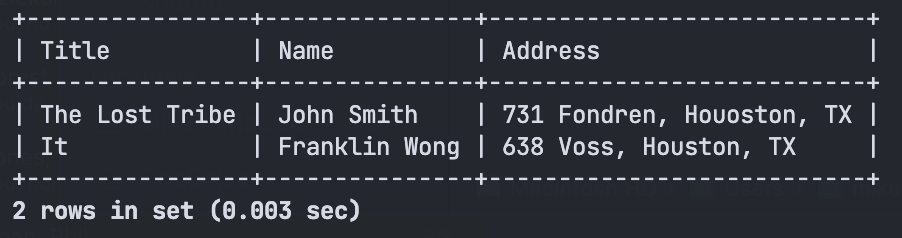
\includegraphics[scale=0.6]{images/q4-d-results.png}
    \caption{Books Loaned on 1/3/2023}
    \label{fig:q4_d_books}
\end{figure}

\subsection{e) For each branch get the number of books loaned}

\textit{For each branch, retrieve the branch name and the total number of books loaned
out from that branch.}

\begin{lstlisting}[language=SQL,
    deletekeywords={IDENTITY},
    deletekeywords={[2]INT},
    morekeywords={clustered},
    framesep=8pt,
    xleftmargin=40pt,
    framexleftmargin=40pt,
    frame=tb,
    framerule=0pt ]
SELECT
    l.Branch_id,
    b.Branch_name,
    COUNT(l.Book_id) AS "Books Loaned"
FROM Book_Loans l
INNER JOIN Library_Branch b
    ON l.Branch_id = b.Branch_id
GROUP BY l.Branch_id; 
\end{lstlisting}

\begin{figure}[!h]
    \centering
    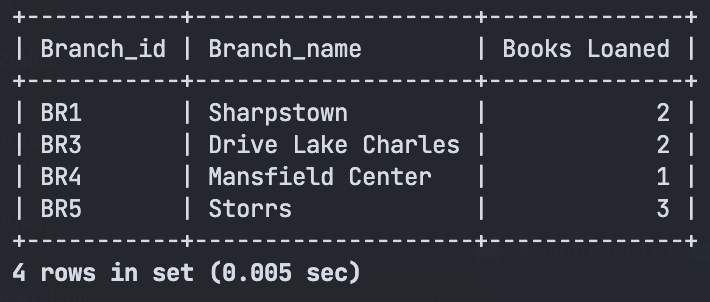
\includegraphics[scale=0.6]{images/q4-e-results.png}
    \caption{Books Loaned by Branch}
    \label{fig:q4_e_books}
\end{figure}

\newpage
\subsection{f) Retrieve info about borrowers with more than two books loaned}

\textit{Retrieve the names, addresses, and number of books checked out for all borrowers who
have more than two books checked out.}

\begin{lstlisting}[language=SQL,
    deletekeywords={IDENTITY},
    deletekeywords={[2]INT},
    morekeywords={clustered},
    framesep=8pt,
    xleftmargin=40pt,
    framexleftmargin=40pt,
    frame=tb,
    framerule=0pt ]
SELECT
    b.Name,
    b.Address,
    COUNT(l.Book_id) AS "Books Out"
FROM Book_Loans l
INNER JOIN Borrower b
    ON l.Card_no = b.Card_no
GROUP BY l.Card_no
HAVING COUNT(*) > 2;
\end{lstlisting}

\begin{figure}[!h]
    \centering
    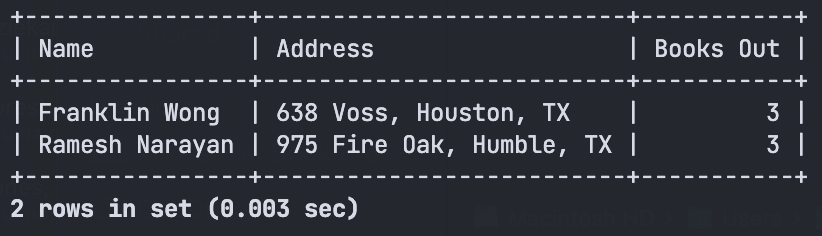
\includegraphics[scale=0.6]{images/q4-f-results.png}
    \caption{Borrowers with More than Two Books Loaned}
    \label{fig:q4_f_borrowers}
\end{figure}

\subsection{g) Retrieve info about books (co)authored by Stephen King at the Central branch}

\textit{For each book authored (or coauthored) by Stephen King, retrieve the title and the
number of copies owned by the `Central' branch.}

\begin{lstlisting}[language=SQL,
    deletekeywords={IDENTITY},
    deletekeywords={[2]INT},
    morekeywords={clustered},
    framesep=8pt,
    xleftmargin=40pt,
    framexleftmargin=40pt,
    frame=tb,
    framerule=0pt ]
SELECT
    b.Title,
    c.No_of_copies
FROM Book_Authors a
INNER JOIN Book b ON
    a.Book_id = b.Book_id   
INNER JOIN Book_Copies c ON
    b.Book_id = c.Book_id
WHERE a.Author_name = "Stephen King" AND c.Branch_id = "BR2";
\end{lstlisting}

\begin{figure}[!h]
    \centering
    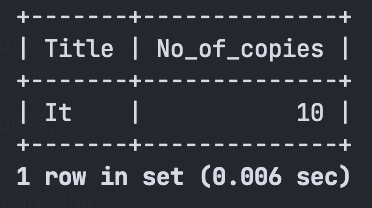
\includegraphics[scale=0.6]{images/q4-g-results.png}
    \caption{Books (Co)Authored by Stephen King at the Central Branch}
    \label{fig:q4_g_books}
\end{figure}

\newpage
\subsection{h) Find books that cannot be loaned on 2/2/2023}

\textit{Assume today is 2/2/2023. Find book(s) that cannot be loaned because all copies in the
library branch have been completely loaned out. Show book title and branch name.}

\begin{lstlisting}[language=SQL,
    deletekeywords={IDENTITY},
    deletekeywords={[2]INT},
    morekeywords={clustered},
    framesep=8pt,
    xleftmargin=40pt,
    framexleftmargin=40pt,
    frame=tb,
    framerule=0pt ]
SELECT
    b.Title,
    p.Branch_name,
    c.No_of_copies
FROM Book_Copies c
INNER JOIN Book b
    ON c.Book_id = b.Book_id
INNER JOIN Book_Loans l
    ON c.Book_id = l.Book_id
        AND c.Branch_id = l.Branch_id
INNER JOIN Library_Branch p
    ON c.Branch_id = p.Branch_id
GROUP BY c.Branch_id
HAVING COUNT(l.Book_id) >= c.No_of_copies; 
\end{lstlisting}

\begin{figure}[!h]
    \centering
    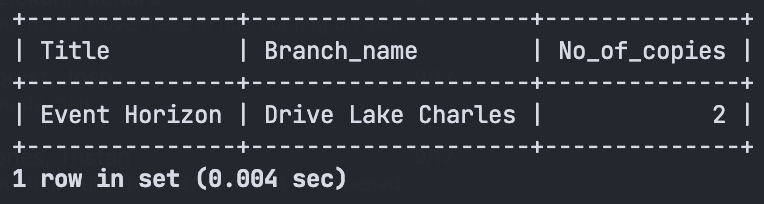
\includegraphics[scale=0.6]{images/q4-h-results.png}
    \caption{Books that Cannot be Loaned on 2/2/2023}
    \label{fig:q4_h_books}
\end{figure}

\subsection{i) Retrieve info about the borrower who loaned all the books by Henry Kissinger}

\textit{Find the name and address of the borrower who loaned all the books authored by Henry
A Kissinger.}

\begin{lstlisting}[language=SQL,
    deletekeywords={IDENTITY},
    deletekeywords={[2]INT},
    morekeywords={clustered},
    framesep=8pt,
    xleftmargin=40pt,
    framexleftmargin=40pt,
    frame=tb,
    framerule=0pt ]
SELECT
    u.Name,
    u.Address
FROM Book_Loans l
INNER JOIN Book b
    ON l.Book_id = b.Book_id
INNER JOIN Borrower u
    ON l.Card_no = u.Card_no
INNER JOIN Book_Authors a
    ON b.Book_id = a.Book_id
WHERE a.Author_name = "Henry A Kissinger"
GROUP BY u.Name
HAVING COUNT(l.Book_id) = (
    SELECT
        COUNT(Book_id)
    FROM
        Book_Authors
    WHERE Author_name = "Henry A Kissinger"
); 
\end{lstlisting}

\begin{figure}[!h]
    \centering
    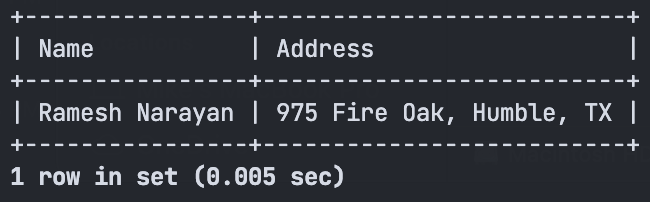
\includegraphics[scale=0.6]{images/q4-i-results.png}
    \caption{Borrower who Loaned all Books by Henry Kissinger}
    \label{fig:q4_i_borrower}
\end{figure}

\newpage
\section{Part 5, Setting Up Constraints}

\subsection{Due Date Validation}

We are able to add a constraint to validate the \textit{Due\_date} column in the \textit{Book\_Loans} table such that a due date cannot be set to occur before the recorded \textit{Date\_out} date.

$\hfill \break$
In order to add it, we can execute the following SQL command to add the constraint to the table:

\begin{lstlisting}[ language=SQL,
    deletekeywords={IDENTITY},
    deletekeywords={[2]INT},
    morekeywords={clustered,load,data,infile,fields,terminated,enclosed,lines},
    framesep=8pt,
    xleftmargin=40pt,
    framexleftmargin=40pt,
    frame=tb,
    framerule=0pt,
    breaklines=true ]
ALTER TABLE Book_Loans ADD CONSTRAINT chk_due_date CHECK (Due_date >= Date_out);
\end{lstlisting}

$\hfill \break$
After adding the constraint, we can verify it was indeed successfully added by using the \textit{SHOW} command to interrogate the table creation command from the system schema. In the below output, we can see on the second to last line of the command our new constraint \textit{chk\_due\_date} was added.

\begin{figure}[!h]
    \centering
    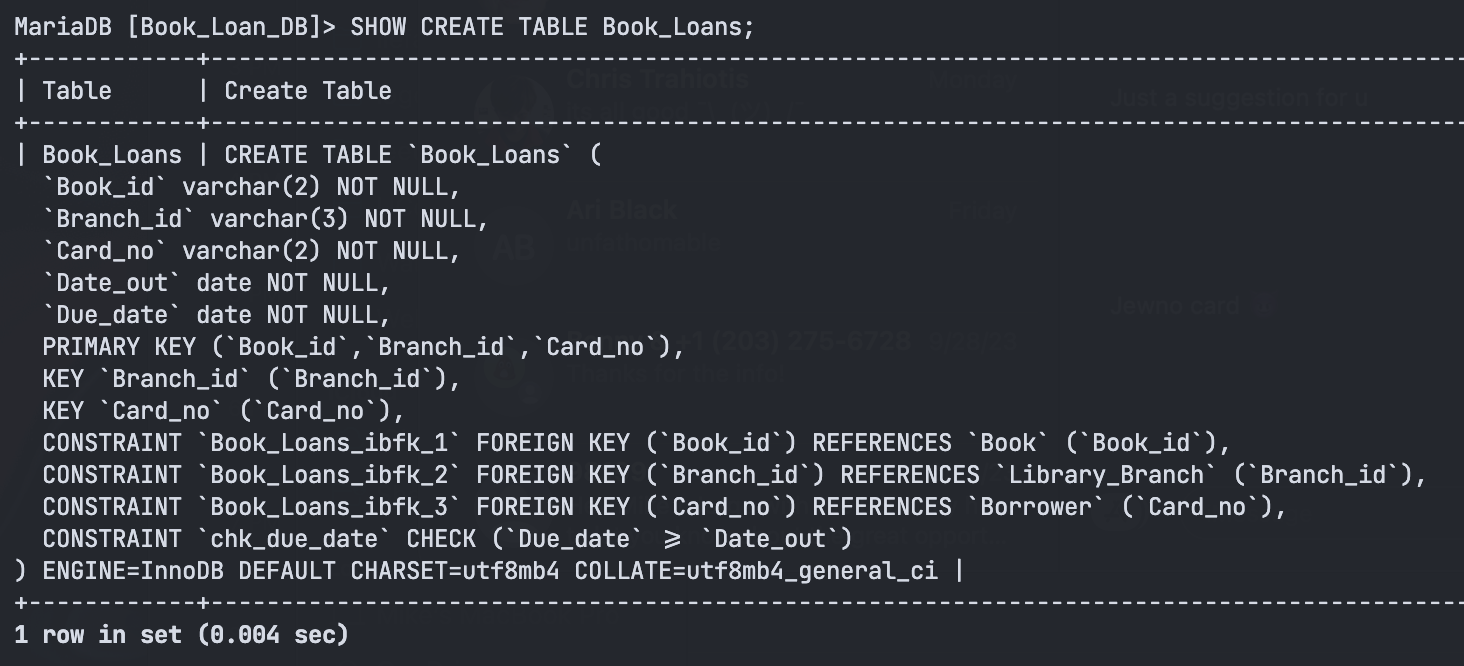
\includegraphics[scale=0.6]{images/q5-constraint-command.png}
    \caption{Constraint Verification}
    \label{fig:q5_a_constraint}
\end{figure}

$\hfill \break$
Now that the constraint is indeed applied to the table, we can try inserting a record with an invalid due date and ensure it fails.

\begin{figure}[!h]
    \centering
    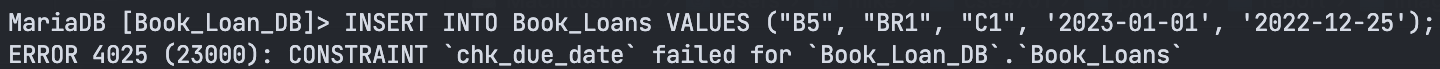
\includegraphics[scale=0.6]{images/q5-constraint-validation.png}
    \caption{Constraint Failure on Invalid Due Date}
    \label{fig:q5_a_invalid_due_date}
\end{figure}

\end{document}